% TikZ source of radial.svg (compile with tectonic; converted with PyMuPDF, text as paths).
\documentclass[tikz,border=4pt]{standalone}
\usepackage{lmodern}
\usepackage{xcolor}
\usetikzlibrary{shapes.geometric}
\definecolor{inkblue}{RGB}{23,65,104}
\begin{document}
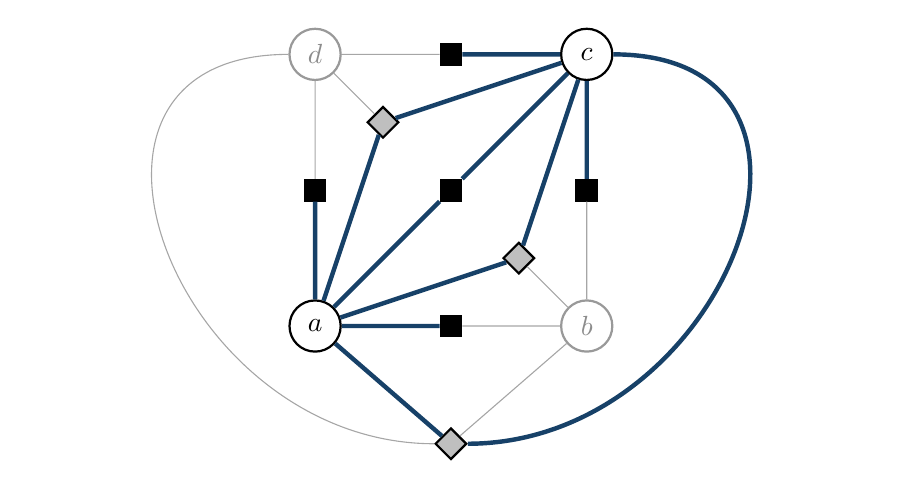
\begin{tikzpicture}[x=1.15cm,y=1.15cm,
 opt/.style={circle,draw,thick,fill=white,minimum size=6.5mm,inner sep=0.5pt},
 optout/.style={circle,draw=black!40,thick,fill=white,text=black!45,minimum size=6.5mm,inner sep=0.5pt},
 term/.style={rectangle,draw,thick,fill=black,minimum size=2.6mm,inner sep=0pt},
 fterm/.style={diamond,draw,thick,fill=black!25,minimum size=4mm,inner sep=0pt},
 hedge/.style={draw=black!35,thin},
 sel/.style={draw=inkblue,line width=1.6pt}]
\node[opt] (a) at (0,0) {$a$};
\node[optout] (b) at (3,0) {$b$};
\node[opt] (c) at (3,3) {$c$};
\node[optout] (d) at (0,3) {$d$};
\node[term] (qab) at (1.5,0) {};
\node[term] (qbc) at (3,1.5) {};
\node[term] (qcd) at (1.5,3) {};
\node[term] (qda) at (0,1.5) {};
\node[term] (qac) at (1.5,1.5) {};
\node[fterm] (f1) at (2.25,0.75) {};
\node[fterm] (f2) at (0.75,2.25) {};
\node[fterm] (fo) at (1.5,-1.3) {};
% edges of H not in H[R u S]
\path[hedge] (qab)--(b) (b)--(qbc) (qcd)--(d) (d)--(qda) (f1)--(b) (f2)--(d) (fo)--(b);
\path[hedge] (fo) to[out=180,in=180,looseness=1.6] (d);
% H[R u S] for the cover S = {a, c}
\path[sel] (a)--(qab) (qbc)--(c) (c)--(qcd) (qda)--(a) (a)--(qac)--(c);
\path[sel] (f1)--(a) (f1)--(c) (f2)--(a) (f2)--(c) (fo)--(a);
\path[sel] (fo) to[out=0,in=0,looseness=1.6] (c);
\end{tikzpicture}
\end{document}
